\documentclass[18pt,compress,dvipdfm]{beamer}
%%%% handoutを指定すると印刷用にフォーマット
% \documentclass[compress,dvipdfm,handout]{beamer}
%%%% しおりが文字化けしないための対策
\AtBeginDvi{\special{pdf:tounicode EUC-UCS2}}
%%%% テーマの指定
% \usetheme{Warsaw}
\usetheme{Antibes}
% \usetheme{Berkeley}
% \usetheme{PaloAlto}
% \usetheme{Berlin}
% \usetheme{Luebeck}
%%%% カラーテーマの指定
% \usecolortheme{lily}
%%%% フォントテーマの指定
\usefonttheme{structurebold}
%%%% 日本語のフォントをゴシックにする
\renewcommand{\kanjifamilydefault}{\gtdefault}
%%%% structureカラーの指定
% \setbeamercolor{structure}{fg=blue!60!black}
%%%% alertカラーの指定
% \setbeamercolor{alerted text}{fg=red!80!black}
\setbeamertemplate{blocks}[rounded]
\setbeamertemplate{navigation symbols}{}
%%%% ロゴを入れる
% \logo{\raisebox{-1.5zw}{\includegraphics[width=5zw]{logo.png}}}
\usepackage{latexsym}
\usepackage{amssymb}
\usepackage{alltt}
\usepackage{wrapfig}
%%%% 後ろで利用しているマクロの定義
\newcommand{\hi}[1]{\temporal<#1>{\color{gray}}{\color{black}}{\color{lightgray}}}
\newcommand{\gotobutton}[1]{\raisebox{-0.15ex}{\beamergotobutton{#1}}}
%%%%%%%%%%%%%%%%%%%%%%%%%%%%%%%%%%%%%%%%%%%%%%%%%%%%%%%%%%%%%%%%
\begin{document}

\title{Ruby-GNOME2のメンテナになってみた話}
\author{@cosmo\_\_}
\date{2013/12/8}
\maketitle

\section{Who am I?}

\begin{frame}
\begin{block}{自己紹介}
{\Large
\begin{wrapfigure}[12]{h}{.3\linewidth}
\begin{center}

\includegraphics[width=3cm]{img/icon.png}
\end{center}
\end{wrapfigure}

TwitterID: @cosmo\_\_

Github: cosmo0920

4月からソフトウェアエンジニアとして働いています

関数型言語好き

Ruby-GNOME2メンテナ(New)

}
\end{block}
\end{frame}

\section{Ruby-GNOME2とは}
\begin{frame}
\begin{block}{Ruby-GNOME2とは}
{\huge
rubyからGTK2/GTK3を使おうとするバインディングライブラリ
}
\end{block}
\end{frame}

\section{Ruby-GNOME2のgemを使っているアプリケーション}
\begin{frame}
\begin{block}{}
{\huge
Q. Ruby-GNOME2のgemを使っているアプリケーションとは?
}
\end{block}
\end{frame}

\section{Ruby-GNOME2のgemを使っているアプリケーション}
\begin{frame}
\begin{block}{}
{\huge
A. mikutter
}
\end{block}
\end{frame}

\section{Ruby-GNOME2と関わったきっかけ}
\begin{frame}
\begin{block}{きっかけ}
\begin{itemize}
{\Large
\item ruby 2.1.0 preview1が出た
\item gtk2入れてmikutterを動かしてみようとした
}
\end{itemize}
\end{block}
\end{frame}

\section{}

\begin{frame}
\begin{center}
{\huge
_人人人人人人人人人人人人人_

> 突然のコンパイルエラー <

 ̄Y\^{}Y\^{}Y\^{}Y\^{}Y\^{}Y\^{}Y\^{}Y\^{}Y\^{}Y\^{}Y ̄
}
\end{center}
\end{frame}

\section{バグ報告をしてみよう}

\begin{itemize}
\item 自分のところだけで直してもいいけれど
\item Upstream(開発元)に報告したほうが他の人も幸せになれる
\item よし、頑張って報告してできたらパッチを書いてみよう
\end{itemize}

\begin{figure}
  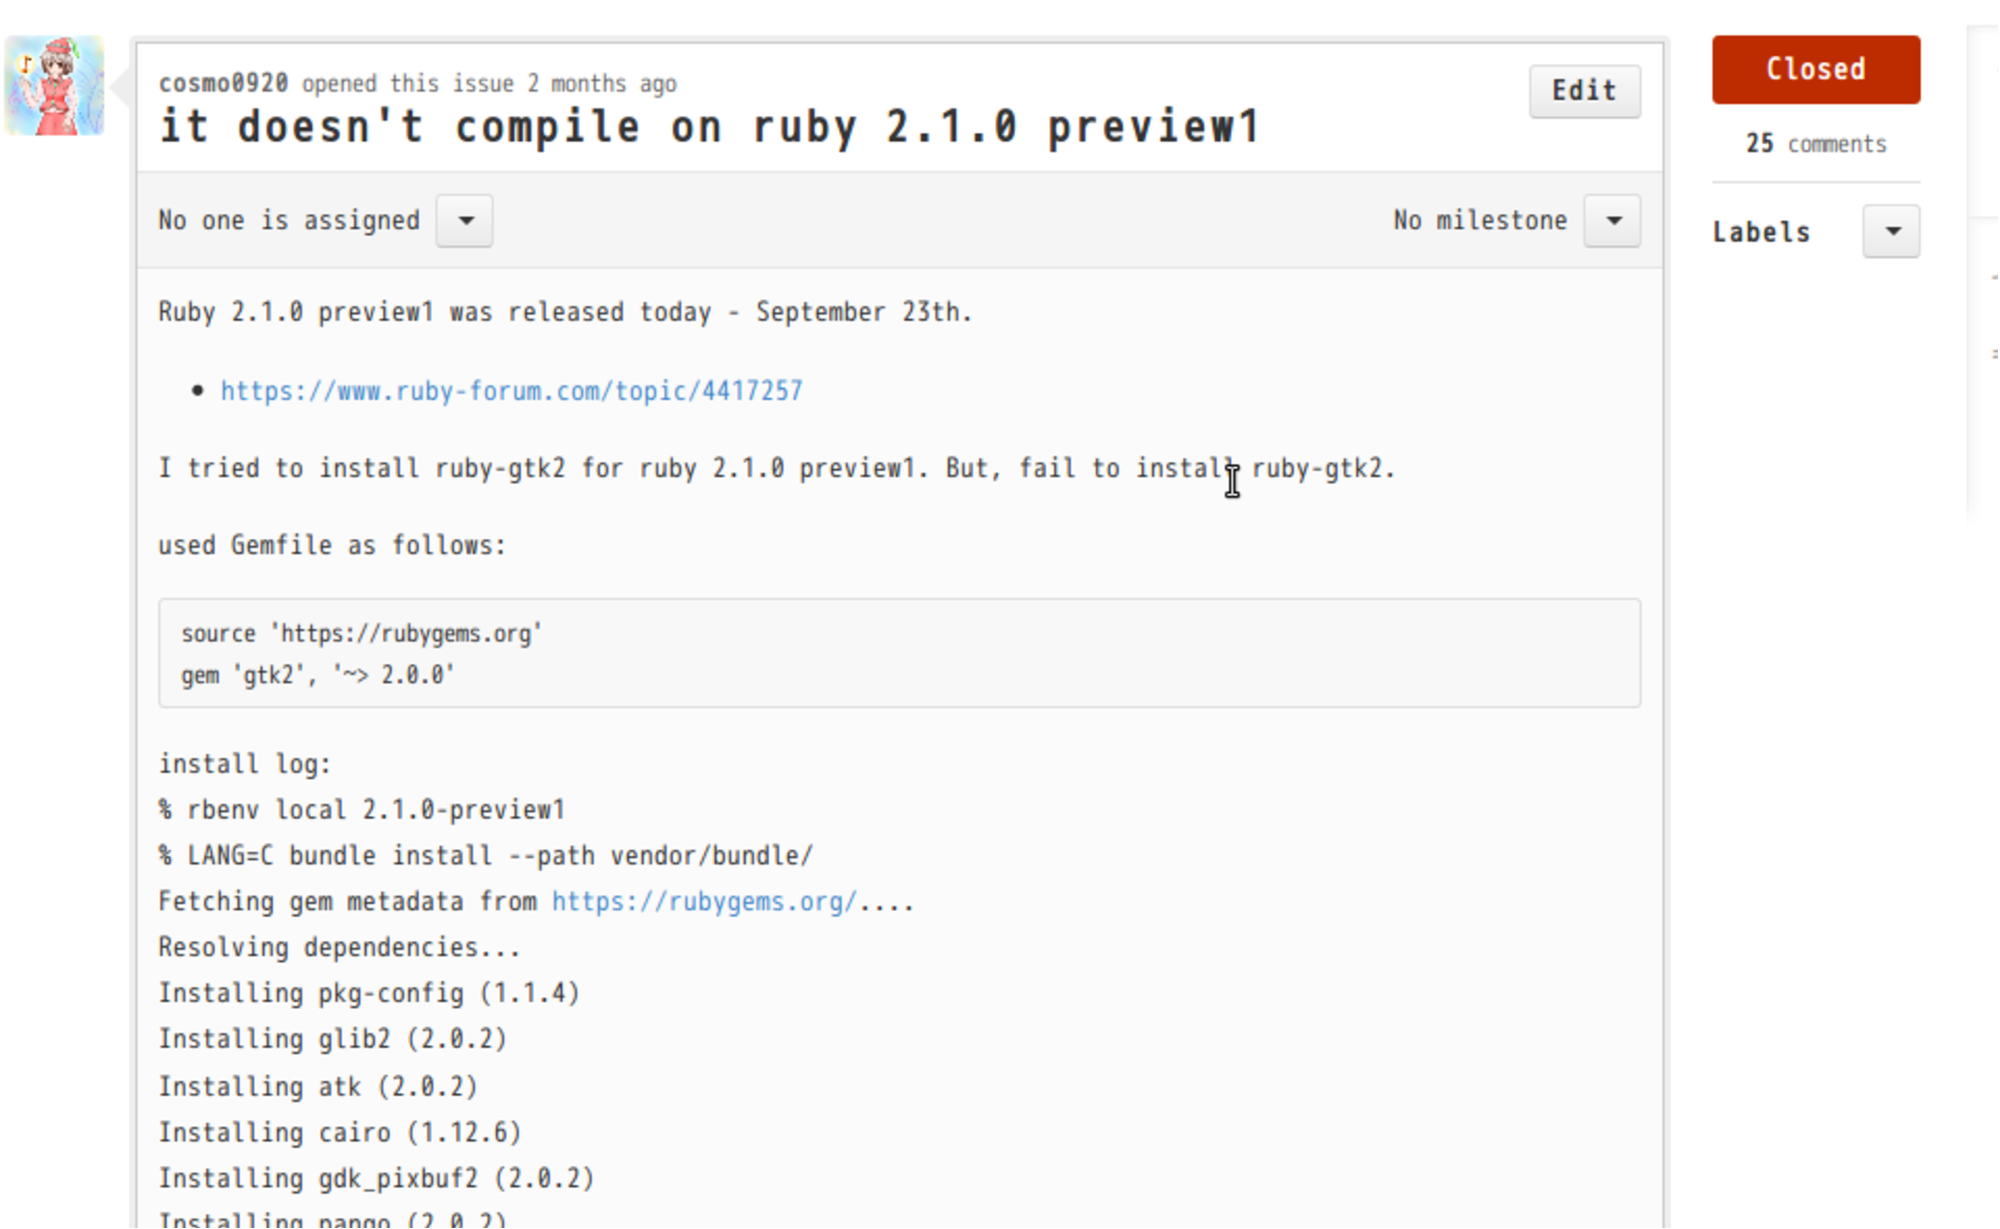
\includegraphics[width=6.5cm]{img/issue180.pdf}
\end{figure}
\section{パッチを投げてみた}

\begin{figure}[h]
\begin{center}
  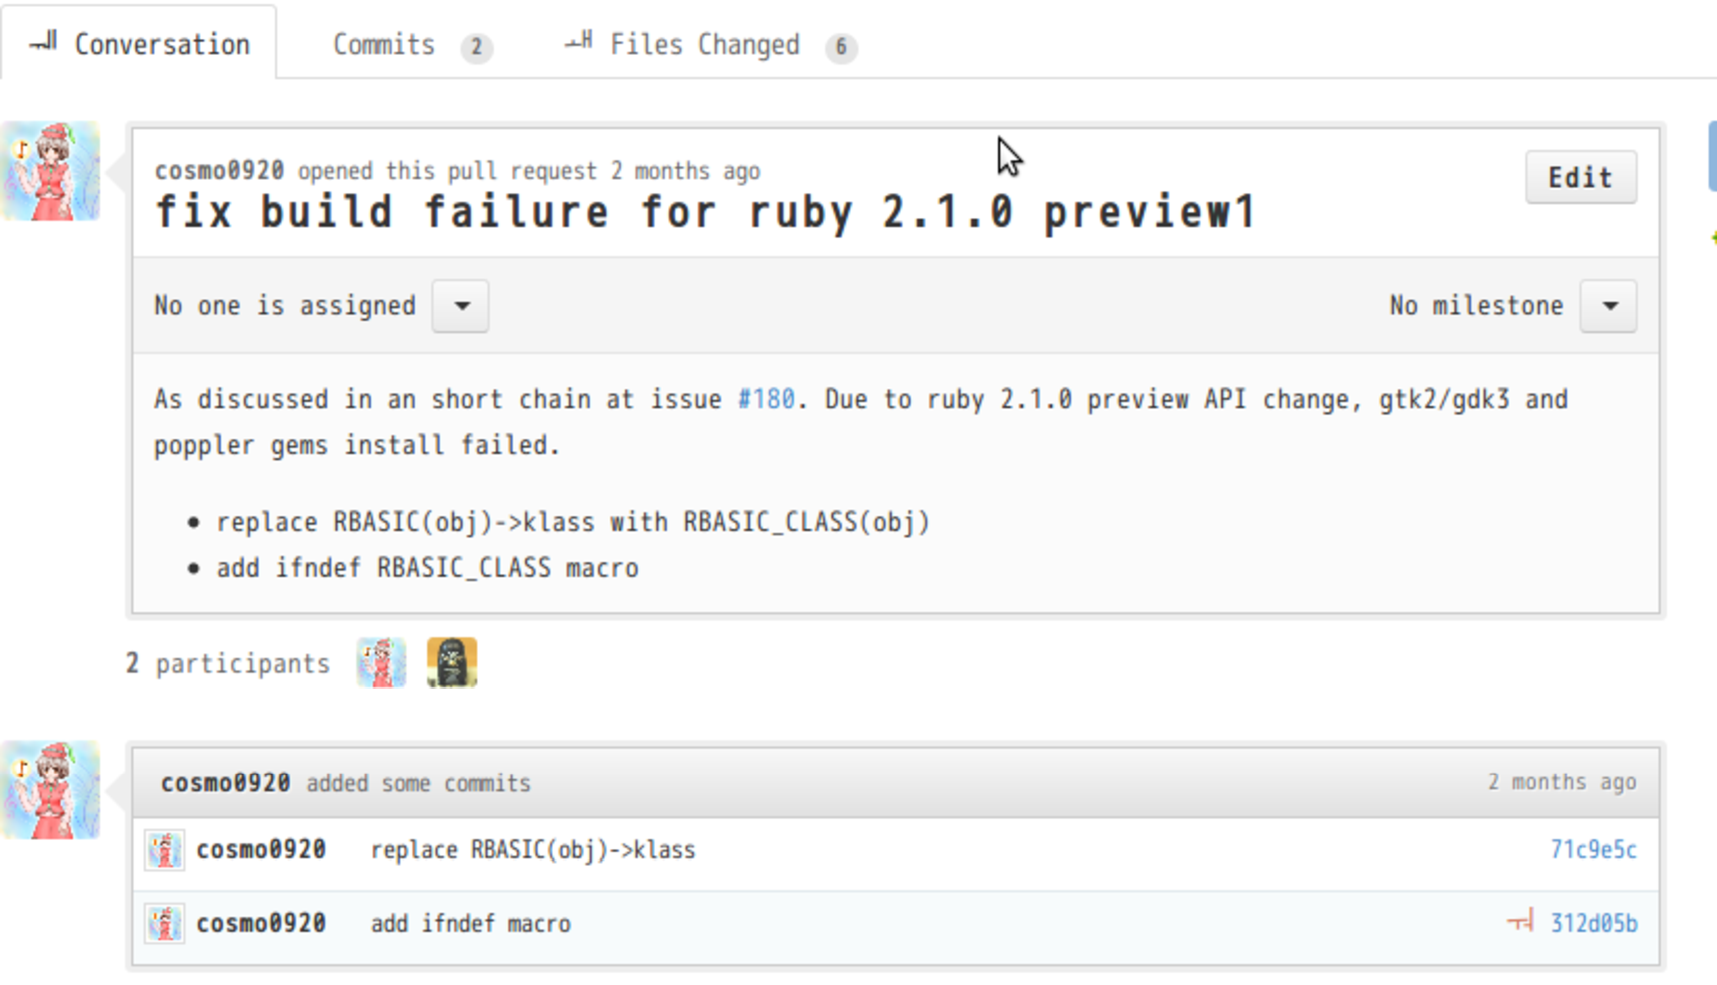
\includegraphics[width=5cm]{img/pull181.pdf}
\end{center}
\end{figure}

\section{その後}

\begin{frame}
\begin{itemize}
\item PullRequestを4件送りました
\item Ruby-GNOME2の開発者にならないかと誘われた
\end{itemize}

→快諾しました
\end{frame}

\section{メンテナとしての自分の方針とか}

\begin{frame}
\begin{itemize}
{\Large
\item 基本的にissueにあがっていることからできそうな所をやってみる方針
\item Ruby-GNOME2のメンバーになった後にMLの存在に気づいた
\item 基本Githubでやり取り、突っ込んだ議論はMLですることも
\item 主にテスト周りのメンテナンスしています
}
\end{itemize}
\end{frame}

\section{メンテナになってからしたこと}

\begin{frame}
\begin{block}{やったことの概要}
\begin{itemize}
{\Large
\item 2.12以前のGTK2のサポートを切る
\item 古いPango/ATK/GLibのサポートを切る
\item rcairoの依存関係の見直し
\item Travis CIを緑にするための作業
\item deprecatedなテストを直す
\item Gdk::EventTouchの実装
\item C言語拡張のコンパイル時の警告への対応
\item GObject-Introspectionを使ったgio2の試験実装
}
\end{itemize}
\end{block}
\end{frame}


\section{Ruby-GNOME2プロジェクトの問題}

\begin{frame}
\begin{itemize}
\item テストコードが少ない事
\item レガシー…

ruby-gtk-0.11 (1998/9〜)

Ruby-GNOME (2001/10〜)

Ruby-GNOME2(〜現在)

\item GUIのライブラリはテストが特に難しい!
\end{itemize}
\end{frame}

\section{Ruby-GNOME2とテストコード}

\begin{frame}
\begin{itemize}
\item RubyUnit(現在のUnit::Test)の0.4.0リリースは2001年09月08日\footnote{http://homepage1.nifty.com/markey/ruby/rubyunit/}
\item GUIのライブラリはテストが特に難しい!
\item それも相まってテストコードが少ない
\end{itemize}
\end{frame}

\section{テスト周りについて}
\begin{frame}
\begin{itemize}
{\huge
\item\hi{1} Ruby-GNOME2ではTest::Unitでテストを書いている
\item\hi{2} GUIのテストは難しい!
\item\hi{3} 労力に見合うだけのテストを書くに留めよう!
\item\hi{4} CIしたいよね!
}
\end{itemize}
\end{frame}

\begin{frame}
\begin{center}
{\Huge
\item 何故テストを書くのか
}
\end{center}
\end{frame}

\begin{frame}
\begin{center}
{\Huge
\item 不安をなくすため?
}
\end{center}
\end{frame}

\begin{frame}
\begin{center}
{\Huge
\item と言うよりも
}
\end{center}
\end{frame}

\begin{frame}
\begin{center}
{\Huge
開発を楽しむため!
}
\end{center}
\end{frame}

\section{テストについて}

\begin{frame}
\begin{itemize}
{\huge
\item\hi{1} 労力に見合うだけのテストを書く
\item\hi{2} テストを書くコストを下げられるなら下げつつ書こう
\item\hi{3} メンテナンスしやすいテストを!
}
\end{itemize}
\end{frame}


\end{document}